%%%%%%%%%%%%%%%%%%%%%%%%%%%%%%%%%%%%%%%%%%%%%%%%%%%%%%%%%%%%%%%%%%%%%%%%%%%%%%%%%
% Template: Article
%
% Por: Abrantes Araújo Silva Filho
%      abrantesasf@gmail.com
%
% Citação: Se você gostou deste template, por favor ajude a divulgá-lo mantendo
%          o link para meu repositório GitHub em:
%          https://github.com/abrantesasf/LaTeX
%%%%%%%%%%%%%%%%%%%%%%%%%%%%%%%%%%%%%%%%%%%%%%%%%%%%%%%%%%%%%%%%%%%%%%%%%%%%%%%%%




%%%%%%%%%%%%%%%%%%%%%%%%%%%%%%%%%%%%%%%%%%%%%%%%%%%%%%%%%%%%%%%%%%%%%%%%%%%%%%%%%
%%% Configura o tipo de documento, papel, tamanho da fonte e informações básicas
%%% para as proriedades do PDF/DVIPS e outras propriedades do documento
\RequirePackage{ifpdf}
\ifpdf
  % Classe, língua e tamanho da fonte padrão. Outras opções a considerar:
  %   draft
  %   onecolumn (padrão) ou twocolumn (OU usar o package multicol)
  %   fleqn com ou sem leqno (alinhamento à esquerda das fórmulas e dos números)
  %   oneside (padrão para article ou report) ou twoside (padrão para book)
  \documentclass[pdftex, brazil, 12pt, oneside]{article}
\else
  % Classe, língua e tamanho da fonte padrão. Outras opções a considerar:
  %   draft
  %   onecolumn (padrão) ou twocolumn (OU usar o package multicol)
  %   fleqn com ou sem leqno (alinhamento à esquerda das fórmulas e dos números)
  %   oneside (padrão para article ou report) ou twoside (padrão para book)
  \documentclass[brazil, 12pt]{article}
\fi


%%%%%%%%%%%%%%%%%%%%%%%%%%%%%%%%%%%%%%%%%%%%%%%%%%%%%%%%%%%%%%%%%%%%%%%%%%%%%%%%%
%%% Carrega pacotes iniciais necessários para estrutura de controle e para a
%%% criação e o parse de novos comandos
\usepackage{ifthen}
\usepackage{xparse}


%%%%%%%%%%%%%%%%%%%%%%%%%%%%%%%%%%%%%%%%%%%%%%%%%%%%%%%%%%%%%%%%%%%%%%%%%%%%%%%%%
%%% Configuração do tamanho da página, margens, espaçamento entrelinhas e, se
%%% necessário, ativa a indentação dos primeiros parágrafos.
\ifpdf
  \usepackage[pdftex]{geometry}
\else
  \usepackage[dvips]{geometry}
\fi
\geometry{a4paper, left=2.0cm, right=2.0cm, top=2.0cm, bottom=2.0cm}

\usepackage{setspace}
  \singlespacing
  %\onehalfspacing
  %\doublespacing


%%%%%%%%%%%%%%%%%%%%%%%%%%%%%%%%%%%%%%%%%%%%%%%%%%%%%%%%%%%%%%%%%%%%%%%%%%%%%%%%%
%%% Configurações de cabeçalho e rodapé:
\usepackage{fancyhdr}
%\setlength{\headheight}{1cm}
%\setlength{\footskip}{1.5cm}
%\renewcommand{\headrulewidth}{0.3pt}
%\renewcommand{\footrulewidth}{0.0pt}
%\pagestyle{fancy}
%\renewcommand{\sectionmark}[1]{%
%  \markboth{\uppercase{#1}}{}}
%\renewcommand{\subsectionmark}[1]{%
%  \markright{\uppercase{\thesubsection \hspace{0.1cm} #1}}{}}
%\fancyhead{}
%\fancyfoot{}
%\newcommand{\diminuifonte}{%
%    \fontsize{9pt}{9}\selectfont
%}
%\newcommand{\aumentafonte}{%
%    \fontsize{12}{12}\selectfont
%}
%% Configura cabeçalho e rodapé para documentos TWOSIDE
%\fancyhead[EL]{\textbf{\thepage}}
%\fancyhead[EC]{}
%\fancyhead[ER]{\diminuifonte \textbf{\leftmark}}
%\fancyhead[OR]{\textbf{\thepage}}
%\fancyhead[OC]{}
%\fancyhead[OL]{\diminuifonte \textbf{\rightmark}}
%\fancyfoot[EL,EC,ER,OR,OC,OL]{}
% Configura cabeçalho e rodapé para documentos ONESIDE
%\lhead{ \fancyplain{}{sup esquerdo} }
%\chead{ \fancyplain{}{sup centro} }
%\rhead{ \fancyplain{}{\thesection} }
%\lfoot{ \fancyplain{}{inf esquerdo} }
%\cfoot{ \fancyplain{}{inf centro} }
%\rfoot{ \fancyplain{}{\thepage} }




%%%%%%%%%%%%%%%%%%%%%%%%%%%%%%%%%%%%%%%%%%%%%%%%%%%%%%%%%%%%%%%%%%%%%%%%%%%%%%%%%
%%% Configurações de encoding, lingua e fontes:
\usepackage[T1]{fontenc}
\usepackage[utf8]{inputenc}
\usepackage{babel}

% Altera a fonte padrão do documento (nem todas funcionam em modo math):
%   phv = Helvetica
%   ptm = Times
%   ppl = Palatino
%   pbk = bookman
%   pag = AdobeAvantGarde
%   pnc = Adobe NewCenturySchoolBook
\renewcommand{\familydefault}{ppl}


%%%%%%%%%%%%%%%%%%%%%%%%%%%%%%%%%%%%%%%%%%%%%%%%%%%%%%%%%%%%%%%%%%%%%%%%%%%%%%%%%
%%% Carrega pacotes para referências cruzadas, citações dentro do documento,
%%% links para internet e outros.Configura algumas opções.
%%% Não altere a ordem de carregamento dos packages.
\usepackage{varioref}
\ifpdf
  \usepackage[pdftex]{hyperref}
    \hypersetup{
      % Informações variáveis em cada documento (MUDE AQUI!):
      pdftitle={Monitoria de Álgebra Linear: revisão de potenciação e radiciação},
      pdfauthor={Abrantes Araújo Silva Filho},
      pdfsubject={Revisão de potências e raízes para alunos de álgebra
                  linear},
      pdfkeywords={potências, raízes, propriedades},
      pdfinfo={
        CreationDate={}, % Ex.: D:AAAAMMDDHH24MISS
        ModDate={}       % Ex.: D:AAAAMMDDHH24MISS
      },
      % Coisas que você não deve alterar se não souber o que está fazendo:
      unicode=true,
      pdflang={pt-BR},
      bookmarksopen=true,
      bookmarksnumbered=true,
      bookmarksopenlevel=5,
      pdfdisplaydoctitle=true,
      pdfpagemode=UseOutlines,
      pdfstartview=FitH,
      pdfcreator={LaTeX with hyperref package},
      pdfproducer={pdfTeX},
      pdfnewwindow=true,
      colorlinks=true,
      citecolor=green,
      linkcolor=red,
      filecolor=cyan,
      urlcolor=blue
    }
\else
  \usepackage{hyperref}
\fi
\usepackage{cleveref}
\usepackage{url}


%%%%%%%%%%%%%%%%%%%%%%%%%%%%%%%%%%%%%%%%%%%%%%%%%%%%%%%%%%%%%%%%%%%%%%%%%%%%%%%%%
%%% Carrega bibliotecas de símbolos (matemáticos, físicos, etc.), fontes
%%% adicionais, e configura algumas opções
\usepackage{amsmath}
\usepackage{amssymb}
\usepackage{amsfonts}
\usepackage{siunitx}
  \sisetup{group-separator = {.}}
  \sisetup{group-digits = {false}}
  \sisetup{output-decimal-marker = {,}}
\usepackage{bm}
\usepackage{cancel}
% Altera separador decimal via comando, se necessário (prefira o siunitx):
%\mathchardef\period=\mathcode`.
%\DeclareMathSymbol{.}{\mathord}{letters}{"3B}
  

%%%%%%%%%%%%%%%%%%%%%%%%%%%%%%%%%%%%%%%%%%%%%%%%%%%%%%%%%%%%%%%%%%%%%%%%%%%%%%%%%
%%% Carrega packages relacionados à computação
\usepackage{algorithm2e}
\usepackage{algorithmicx}
\usepackage{algpseudocode}
\usepackage{listings}
  \lstset{literate=
    {á}{{\'a}}1 {é}{{\'e}}1 {í}{{\'i}}1 {ó}{{\'o}}1 {ú}{{\'u}}1
    {Á}{{\'A}}1 {É}{{\'E}}1 {Í}{{\'I}}1 {Ó}{{\'O}}1 {Ú}{{\'U}}1
    {à}{{\`a}}1 {è}{{\`e}}1 {ì}{{\`i}}1 {ò}{{\`o}}1 {ù}{{\`u}}1
    {À}{{\`A}}1 {È}{{\'E}}1 {Ì}{{\`I}}1 {Ò}{{\`O}}1 {Ù}{{\`U}}1
    {ä}{{\"a}}1 {ë}{{\"e}}1 {ï}{{\"i}}1 {ö}{{\"o}}1 {ü}{{\"u}}1
    {Ä}{{\"A}}1 {Ë}{{\"E}}1 {Ï}{{\"I}}1 {Ö}{{\"O}}1 {Ü}{{\"U}}1
    {â}{{\^a}}1 {ê}{{\^e}}1 {î}{{\^i}}1 {ô}{{\^o}}1 {û}{{\^u}}1
    {Â}{{\^A}}1 {Ê}{{\^E}}1 {Î}{{\^I}}1 {Ô}{{\^O}}1 {Û}{{\^U}}1
    {œ}{{\oe}}1 {Œ}{{\OE}}1 {æ}{{\ae}}1 {Æ}{{\AE}}1 {ß}{{\ss}}1
    {ű}{{\H{u}}}1 {Ű}{{\H{U}}}1 {ő}{{\H{o}}}1 {Ő}{{\H{O}}}1
    {ç}{{\c c}}1 {Ç}{{\c C}}1 {ø}{{\o}}1 {å}{{\r a}}1 {Å}{{\r A}}1
    {€}{{\euro}}1 {£}{{\pounds}}1 {«}{{\guillemotleft}}1
    {»}{{\guillemotright}}1 {ñ}{{\~n}}1 {Ñ}{{\~N}}1 {¿}{{?`}}1
  }
  

%%%%%%%%%%%%%%%%%%%%%%%%%%%%%%%%%%%%%%%%%%%%%%%%%%%%%%%%%%%%%%%%%%%%%%%%%%%%%%%%%
%%% Ativa suporte extendido a cores
\usepackage[svgnames]{xcolor} % Opções de cores: usenames (16), dvipsnames (64),
                              % svgnames (150) e x11names (300).


%%%%%%%%%%%%%%%%%%%%%%%%%%%%%%%%%%%%%%%%%%%%%%%%%%%%%%%%%%%%%%%%%%%%%%%%%%%%%%%%%
%%% Suporte à importação de gráficos externos
\ifpdf
  \usepackage[pdftex]{graphicx}
\else
  \usepackage[dvips]{graphicx}
\fi


%%%%%%%%%%%%%%%%%%%%%%%%%%%%%%%%%%%%%%%%%%%%%%%%%%%%%%%%%%%%%%%%%%%%%%%%%%%%%%%%%
%%% Suporte à criação de gráficos proceduralmente na LaTeX:
\usepackage{tikz}
  \usetikzlibrary{arrows,automata,backgrounds,matrix,patterns,positioning,shapes,shadows}


%%%%%%%%%%%%%%%%%%%%%%%%%%%%%%%%%%%%%%%%%%%%%%%%%%%%%%%%%%%%%%%%%%%%%%%%%%%%%%%%%
%%% Packages para tabelas
\usepackage{array}
\usepackage{longtable}
\usepackage{tabularx}
\usepackage{tabu}
\usepackage{lscape}
\usepackage{colortbl}  
\usepackage{booktabs}


%%%%%%%%%%%%%%%%%%%%%%%%%%%%%%%%%%%%%%%%%%%%%%%%%%%%%%%%%%%%%%%%%%%%%%%%%%%%%%%%%
%%% Packages ambientes de listas
\usepackage{enumitem}
\usepackage[ampersand]{easylist}


%%%%%%%%%%%%%%%%%%%%%%%%%%%%%%%%%%%%%%%%%%%%%%%%%%%%%%%%%%%%%%%%%%%%%%%%%%%%%%%%%
%%% Packages para suporte a ambientes floats, captions, etc.:
\usepackage{float}
\usepackage{wrapfig}
\usepackage{placeins}
\usepackage{caption}
\usepackage{sidecap}
\usepackage{subcaption}


%%%%%%%%%%%%%%%%%%%%%%%%%%%%%%%%%%%%%%%%%%%%%%%%%%%%%%%%%%%%%%%%%%%%%%%%%%%%%%%%%
%%% Meus comandos específicos:
% Commando para ``italizar´´ palavras em inglês (e outras línguas!):
\newcommand{\ingles}[1]{\textit{#1}}

% Commando para colocar o espaço correto entre um número e sua unidade:
\newcommand{\unidade}[2]{\ensuremath{#1\,\mathrm{#2}}}
\newcommand{\unidado}[2]{{#1}\,{#2}}

% Produz ordinal masculino ou feminino dependendo do segundo argumento:
\newcommand{\ordinal}[2]{%
#1%
\ifthenelse{\equal{a}{#2}}%
{\textordfeminine}%
{\textordmasculine}}


%%%%%%%%%%%%%%%%%%%%%%%%%%%%%%%%%%%%%%%%%%%%%%%%%%%%%%%%%%%%%%%%%%%%%%%%%%%%%%%%%
%%% Hifenização específica quando o LaTeX/Babel não conseguirem hifenizar:
\babelhyphenation{Git-Hub}

\usepackage[most]{tcolorbox}

\tcbset{colback=yellow!10!white, colframe=red!50!black, 
        highlight math style= {enhanced, %<-- needed for the ’remember’ options
            colframe=red,colback=red!10!white,boxsep=0pt}
        }
%%%%%%%%%%%%%%%%%%%%%%%%%%%%%%%%%%%%%%%%%%%%%%%%%%%%%%%%%%%%%%%%%%%%%%%%%%%%%%%%%
%%%%%%%%%%%%%%%%%%%%%%%%%%%%%%%%%%%%%%%%%%%%%%%%%%%%%%%%%%%%%%%%%%%%%%%%%%%%%%%%%
%%%%%%%%%%%%%%%%%%%%%%%%%%%%%%%%%%%%%%%%%%%%%%%%%%%%%%%%%%%%%%%%%%%%%%%%%%%%%%%%%
%%%%%%%%%%%%%%%%%%%%%%%%%%%%%%%%%%%%%%%%%%%%%%%%%%%%%%%%%%%%%%%%%%%%%%%%%%%%%%%%%
%%%%%%%%%%%%%%%%%%%%%%%%%%%%%% COMEÇA O DOCUMENTO %%%%%%%%%%%%%%%%%%%%%%%%%%%%%%%
%%%%%%%%%%%%%%%%%%%%%%%%%%%%%%%%%%%%%%%%%%%%%%%%%%%%%%%%%%%%%%%%%%%%%%%%%%%%%%%%%
%%%%%%%%%%%%%%%%%%%%%%%%%%%%%%%%%%%%%%%%%%%%%%%%%%%%%%%%%%%%%%%%%%%%%%%%%%%%%%%%%
%%%%%%%%%%%%%%%%%%%%%%%%%%%%%%%%%%%%%%%%%%%%%%%%%%%%%%%%%%%%%%%%%%%%%%%%%%%%%%%%%
%%%%%%%%%%%%%%%%%%%%%%%%%%%%%%%%%%%%%%%%%%%%%%%%%%%%%%%%%%%%%%%%%%%%%%%%%%%%%%%%%
\begin{document}
\title{Revisão sobre potenciação e radiciação}
\author{Abrantes Araújo Silva Filho}
\date{2019-04-05}
\maketitle
\tableofcontents
%\newpage




%%%%%%%%%%%%%%%%%%%%%%%%%%%%%%%%%%%%%%%%%%%%%%%%%%%%%%%%%%%%%%%%%%%%%%%%%%%%%%%%%
%%%%%%%%%%%%%%%%%%%%%%%%%%%%%%%%%%%%%%%%%%%%%%%%%%%%%%%%%%%%%%%%%%%%%%%%%%%%%%%%%
%%%%%%%%%%%%%%%%%%%%%%%%%%%%%%%%%%%%%%%%%%%%%%%%%%%%%%%%%%%%%%%%%%%%%%%%%%%%%%%%%
\section{Introdução}
\label{intro}

Esta documento é uma revisão geral das propriedades da
\emph{potenciação} e da \emph{radiciação} para os alunos da disciplina
de Álgebra Linear e Geometria Analítica, durante as atividades de
monitoria.

Como o esperado é que os alunos já saibam esse conteúdo, não reescrevi
toda a teoria de potências ou raízes, apenas preparei uma compilação
com todas as propriedades que os alunos \emph{devem dominar} para o
sucesso na Álgebra Linear\footnote{E em outras disciplinas também,
  como cálculo, física, matemática discreta e outras.}, e uma lista de
exercícios a respeito dessas propriedades.

Espera-se que os alunos dominem as propriedades listadas aqui e façam
os exercícios correspondentes. A correção dos exercícios, explicações
extras e esclarecimento de dúvidas, serão realizadas nas atividades de
monitoria.

CUIDADO: preste muita atenção aos detalhes de quando uma propriedade
se aplica, por exemplo: existe uma propriedade que diz que qualquer
número elevado a 0 é igual a 1 ($a^0 = 1$), mas essa propriedade só é
valida se $a \ne 0$. Preste atenção nesses detalhes para não aplicar
uma propriedade de forma errada!

Críticas e sugestões, favor entrar em contato através do e-mail:
\url{abrantesasf@gmail.com}. Obrigado!




%%%%%%%%%%%%%%%%%%%%%%%%%%%%%%%%%%%%%%%%%%%%%%%%%%%%%%%%%%%%%%%%%%%%%%%%%%%%%%%%%
%%%%%%%%%%%%%%%%%%%%%%%%%%%%%%%%%%%%%%%%%%%%%%%%%%%%%%%%%%%%%%%%%%%%%%%%%%%%%%%%%
%%%%%%%%%%%%%%%%%%%%%%%%%%%%%%%%%%%%%%%%%%%%%%%%%%%%%%%%%%%%%%%%%%%%%%%%%%%%%%%%%
\section{Potenciação}
\label{potenciacao}

A \emph{potenciação}, ou exponenciação, é uma operação matemática que
representa um número multiplicado por ele mesmo, várias vezes. Assim:

\begin{tcolorbox}[ams equation]
  a^n = \underbrace{a \times a \times a \times \cdots \times
    a}_{n{\mbox{ vezes}}} = b
\end{tcolorbox}

Por exemplo: $2^3 = 2 \times 2 \times 2 = 8$.

A nomenclatura correta para uma potenciação, $a^n = b$, é:

\begin{itemize}
\item \emph{Base}: é o número que está sendo multiplicado por ele
  mesmo ($a$);
\item \emph{Expoente}\footnote{Cuidado: muita gente escreve expoNente,
  erroneamente. O correto é expOEnte!}: é o número de vezes ($n$) que a base
  é multiplicada por ela mesma; e
\item \emph{Potência}: é o resultado do produto ($b$).
\end{itemize}


%%%%%%%%%%%%%%%%%%%%%%%%%%%%%%%%%%%%%%%%%%%%%%%%%%%%%%%%%%%%%%%%%%%%%%%%%%%%%%%%%
%%%%%%%%%%%%%%%%%%%%%%%%%%%%%%%%%%%%%%%%%%%%%%%%%%%%%%%%%%%%%%%%%%%%%%%%%%%%%%%%%
\subsection{Propriedades da potenciação com expoente inteiro}
\label{potenciacao-propriedades}

As propriedades da potenciação com expoente inteiro\footnote{Potências
com expoentes racionais serão vistas na Seção~\ref{potrad}.} estão listadas a seguir. Preste atenção
às condições nas quais cada propriedade se aplica!

Todo número elevado a $0$ é 1:
\begin{tcolorbox}[ams equation]
  \label{eqn:pot0}
  a^0 = 1\quad (\text{para}\ a \ne 0)
\end{tcolorbox}

Por causa da condição na equação~\ref{eqn:pot0}, não existe $0^0$:
\begin{tcolorbox}[ams equation]
  0^0 = \nexists
\end{tcolorbox}

Cuidado com potências de números negativos:
\begin{tcolorbox}[ams equation]
  \label{eqn:pot-negativ1}
  -a^n = -(a^n) = -\left(\underbrace{a \times a \times a \times
    \cdots \times a}_{n{\mbox{ vezes}}}\right) = -b
\end{tcolorbox}

\begin{tcolorbox}[ams equation]
  \label{eqn:pot-negativ2}
  (-a)^n = \underbrace{(-a) \times (-a) \times (-a) \times
    \cdots \times (-a)}_{n{\mbox{ vezes}}} = \begin{cases}
    +b & \text{se}\ n\ \text{for par}\\
    -b & \text{se}\ n\ \text{for ímpar}
  \end{cases}
\end{tcolorbox}

Produto de potências de mesma base:
\begin{tcolorbox}[ams equation]
  \label{equn:prod_pot}
  a^n \times a^m = a^{n+m}
\end{tcolorbox}

\newpage
Divisão de potências de mesma base (todo mundo se lembra da
propriedade na equação~\ref{eqn:div_pot1}, mas a propriedade na
equação~\ref{eqn:div_pot2} é equivalente e útil em algumas situações):
\begin{tcolorbox}[ams equation]
  \label{eqn:div_pot1}
  \frac{a^n}{a^m} = a^{n-m}\quad (a \ne 0)
\end{tcolorbox}

\begin{tcolorbox}[ams equation]
  \label{eqn:div_pot2}
  \frac{a^n}{a^m} = \frac{1}{a^{m-n}}\quad (a \ne 0)
\end{tcolorbox}

Potência de uma potência:
\begin{tcolorbox}[ams equation]
  \label{eqn:pot_pot}
  (a^n)^m = a^{nm}
\end{tcolorbox}

Potência de um produto:
\begin{tcolorbox}[ams equation]
  \label{eqn:pot_prod}
  (ab)^n = a^nb^n
\end{tcolorbox}

Potência de um quociente:
\begin{tcolorbox}[ams equation]
  \label{eqn:pot_div}
  \left(\frac{a}{b}\right)^n = \frac{a^n}{b^n}\quad (b \ne 0)
\end{tcolorbox}

Potência com expoente negativo:
\begin{tcolorbox}[ams equation]
  \label{eqn:pot_exponegat1}
  a^{-n} = \left(\frac{1}{a}\right)^n = \frac{1^n}{a^n} =
  \frac{1}{a^n}\quad (a \ne 0)
\end{tcolorbox}

\begin{tcolorbox}[ams equation]
  \label{eqn:pot_exponegat2}
  \left(\frac{a}{b}\right)^{-n} = \left(\frac{b}{a}\right)^n =
  \frac{b^n}{a^n}\quad (a \ne 0)
\end{tcolorbox}

Potência com um expoente que é uma potência:
\begin{tcolorbox}[ams equation]
  \label{eqn:pot_pot_pot}
  a^{b^c} = a^{(b^c)}
\end{tcolorbox}




%%%%%%%%%%%%%%%%%%%%%%%%%%%%%%%%%%%%%%%%%%%%%%%%%%%%%%%%%%%%%%%%%%%%%%%%%%%%%%%%%
%%%%%%%%%%%%%%%%%%%%%%%%%%%%%%%%%%%%%%%%%%%%%%%%%%%%%%%%%%%%%%%%%%%%%%%%%%%%%%%%%
%%%%%%%%%%%%%%%%%%%%%%%%%%%%%%%%%%%%%%%%%%%%%%%%%%%%%%%%%%%%%%%%%%%%%%%%%%%%%%%%%
\section{Radiciação}
\label{radiciacao}

A \emph{radiciação}, infelizmente, é uma operação difícil de se
descrever em palavras, portanto preste atenção!

A radiciação é uma
operação que realizamos quando temos um número conhecido e
queremos descobrir que outro número que, multiplicado por ele mesmo
uma determinada quantidades de vezes, resulta no valor que
conhecemos. Alguns exemplos talvez facilitem:

\begin{itemize}
\item Eu tenho o número $125$ e desejo descobrir que
  outro número, multiplicado por ele mesmo $3$ vezes, resulta em
  $125$. Ou seja, quero descobrir o número $x$, tal que $x^3 = 125$;
\item Eu tenho o número $125$ e desejo descobrir que outro
  número, multiplicado por ele mesmo $4$ vezes, resulta em $125$. Ou
  seja, quero descobrir o número $x$, tal que $x^4 = 125$.
\end{itemize}

Em termos mais formais: se $n$ é um inteiro positivo e se $x^n = a$,
então $x$ é dito a $n$-ésima raiz de $a$. Em particular, $x$ é chamado
de raiz quadrada de $a$ se $x^2 = a$, e chamado de raiz cúbica de $a$
se $x^3 = a$.

Para indicar a radiciação usamos um símbolo especial:

\begin{tcolorbox}[ams equation]
  \label{eqn:def_radiciacao}
  \sqrt[n]{a} = x\quad (\text{ou seja:}\ x^n = a)
\end{tcolorbox}

Entendendo corretamente a notação:
\begin{itemize}
  \item \emph{Símbolo da radiciação}: é o símbolo $\sqrt{\text{\ \ }}$, e indica
    que estamos realizando uma operação de radiciação;
  \item \emph{Índice do radical}: é o número $n$ colocado acima do
    símbolo da radiciação, e indica quantas vezes o número que
    estamos procurando foi multiplicado por ele mesmo;
  \item \emph{Radicando}: é o número $a$ que conhecemos, é o resultado da
    multiplicação do número que estamos procurando.
\end{itemize}

Note que, por convenção, quando estamos querendo buscar a raiz
quadrada (índice $n = 2$), não é necessário escrever o índice sobre o
sinal da radiciação. Assim, $\sqrt[2]{a} = \sqrt{a}$, por convenção.


%%%%%%%%%%%%%%%%%%%%%%%%%%%%%%%%%%%%%%%%%%%%%%%%%%%%%%%%%%%%%%%%%%%%%%%%%%%%%%%%%
%%%%%%%%%%%%%%%%%%%%%%%%%%%%%%%%%%%%%%%%%%%%%%%%%%%%%%%%%%%%%%%%%%%%%%%%%%%%%%%%%
\subsection{Propriedades da radiciação}
\label{radiciacao-propriedades}

As propriedades da radiciação estão listadas a seguir. Preste atenção
às condições nas quais cada propriedade se aplica!

Raiz n-ésima de um número elevado à n-ésima potência:
\begin{tcolorbox}[ams equation]
  \label{eqn:nesima_raiz_nesima_pot}
  \sqrt[n]{a^n} = \begin{cases}
    |a| & \text{se}\ a \in \mathbb{R}, n \in \mathbb{N}, n =
    \text{par}\\
    a   & \text{se}\ a \in \mathbb{R}, n \in \mathbb{N}, n = \text{ímpar}
  \end{cases}
\end{tcolorbox}

Alteração do índice através de multiplicação ou divisão:
\begin{tcolorbox}[ams equation]
  \label{eqn:raiz_prod_ind}
  \sqrt[n]{a^m} = \sqrt[n \cdot p]{a^{m \cdot p}}\quad (a \in
  \mathbb{R}, (n, p) \in \mathbb{N} > 1)
\end{tcolorbox}

\begin{tcolorbox}[ams equation]
  \label{eqn:raiz_div_ind}
  \sqrt[n]{a^m} = \sqrt[n : p]{a^{m : p}}\quad (a \in
  \mathbb{R}, (n, p) \in \mathbb{N} > 1)
\end{tcolorbox}

Raiz de um produto:
\begin{tcolorbox}[ams equation]
  \label{eqn:mult_raizes}
  \sqrt[n]{ab} = \sqrt[n]{a} \times \sqrt[n]{b}\quad \begin{cases}
    n \in \mathbb{N} > 1, (a, b) \in \mathbb{R}\\
    \text{se}\ (a, b) \ge 0, n\ \text{deve ser par}
  \end{cases}
\end{tcolorbox}

Raiz de um quociente:
\begin{tcolorbox}[ams equation]
  \label{eqn:div_raizes}
  \sqrt[n]{\frac{a}{b}} = \frac{\sqrt[n]{a}}{\sqrt[n]{b}}\quad (n \in
  \mathbb{N} > 1, (a, b) \in \mathbb{R}, b \ne 0)
\end{tcolorbox}

\newpage
Potência de uma raiz:
\begin{tcolorbox}[ams equation]
  \label{eqn:pot_raiz}
  \left(\sqrt[n]{a^m}\right)^k = \sqrt[n]{a^{mk}}
\end{tcolorbox}

Raiz de uma raiz:
\begin{tcolorbox}[ams equation]
  \label{eqn:raiz_raiz}
  \sqrt[n]{\sqrt[k]{a}} = \sqrt[nk]{a}
\end{tcolorbox}

Multiplicação de radicais com índices diferentes:
\begin{tcolorbox}[ams equation]
  \label{eqn:mult_raiz_indice_diferente}
  \sqrt[n]{a^m} \times \sqrt[p]{b^k} = \sqrt[MMC(n,
    p)]{a^{\frac{MMC(n,p)}{n}m}} \times \sqrt[MMC(n,
    p)]{b^{\frac{MMC(n,p)}{p}k}} = \sqrt[MMC(n,
    p)]{a^{\frac{MMC(n,p)}{n}m}b^{\frac{MMC(n,p)}{p}k}}
\end{tcolorbox}

Divisão de radicais com índices diferentes:
\begin{tcolorbox}[ams equation]
  \label{eqn:div_raiz_indice_diferente}
  \frac{\sqrt[n]{a^m}}{\sqrt[p]{b^k}} =
  \frac{\sqrt[MMC(n,p)]{a^{\frac{MMC(n,p)}{n}m}}}{\sqrt[MMC(n,
      p)]{b^{\frac{MMC(n,p)}{p}k}}} =
  \sqrt[MMC(n,
    p)]{\frac{a^{\frac{MMC(n,p)}{n}m}}{b^{\frac{MMC(n,p)}{p}k}}}
\end{tcolorbox}


%%%%%%%%%%%%%%%%%%%%%%%%%%%%%%%%%%%%%%%%%%%%%%%%%%%%%%%%%%%%%%%%%%%%%%%%%%%%%%%%%
%%%%%%%%%%%%%%%%%%%%%%%%%%%%%%%%%%%%%%%%%%%%%%%%%%%%%%%%%%%%%%%%%%%%%%%%%%%%%%%%%
\subsection{Situações especiais}
\label{radiciacao-especiais}

É necessário ficar atento à algumas situações e casos especiais da
radiciação:

\begin{itemize}
  \item Se $a \ge 0$ e $n = (\text{par ou ímpar})$, $\sqrt[n]{a} \ge 0$;
  \item Se $a < 0$ e $n = \text{par}$, $\sqrt[n]{a} \notin \mathbb{R}$;
  \item Se $a < 0$ e $n = \text{ímpar}$, $\sqrt[n]{a} < 0$;
    \item $\sqrt[1]{a} = a$;
  \item $\sqrt[0]{a}$ não tem sentido matemático; e
    \item Todo número $a > 0$ tem duas raízes quadradas, numericamente
      iguais mas opostas em sinal: a raiz positiva é dita raiz
      principal, e é a essa raiz que estamos nos referindo quando
      falamos $\sqrt{a}$.
\end{itemize}




%%%%%%%%%%%%%%%%%%%%%%%%%%%%%%%%%%%%%%%%%%%%%%%%%%%%%%%%%%%%%%%%%%%%%%%%%%%%%%%%%
%%%%%%%%%%%%%%%%%%%%%%%%%%%%%%%%%%%%%%%%%%%%%%%%%%%%%%%%%%%%%%%%%%%%%%%%%%%%%%%%%
%%%%%%%%%%%%%%%%%%%%%%%%%%%%%%%%%%%%%%%%%%%%%%%%%%%%%%%%%%%%%%%%%%%%%%%%%%%%%%%%%
\section{Potencias \emph{versus} Raízes: são funções inversas}
\label{potrad}

Como você já sabe, a potenciação é a operação \emph{inversa} da
radiciação, e vice-versa. Assim, dada uma função de potenciação, por
exemplo $y = x^3$, a função inversa será $x = \sqrt[3]{y}$ (veja a
figura a seguir):

\begin{figure}[H]
  \begin{center}
    \caption{$y=x^3$ é a inversa de $x=\sqrt[3]{y}$ (e vice-versa)}
    \label{fig:pot-rad-inv}
    \fbox{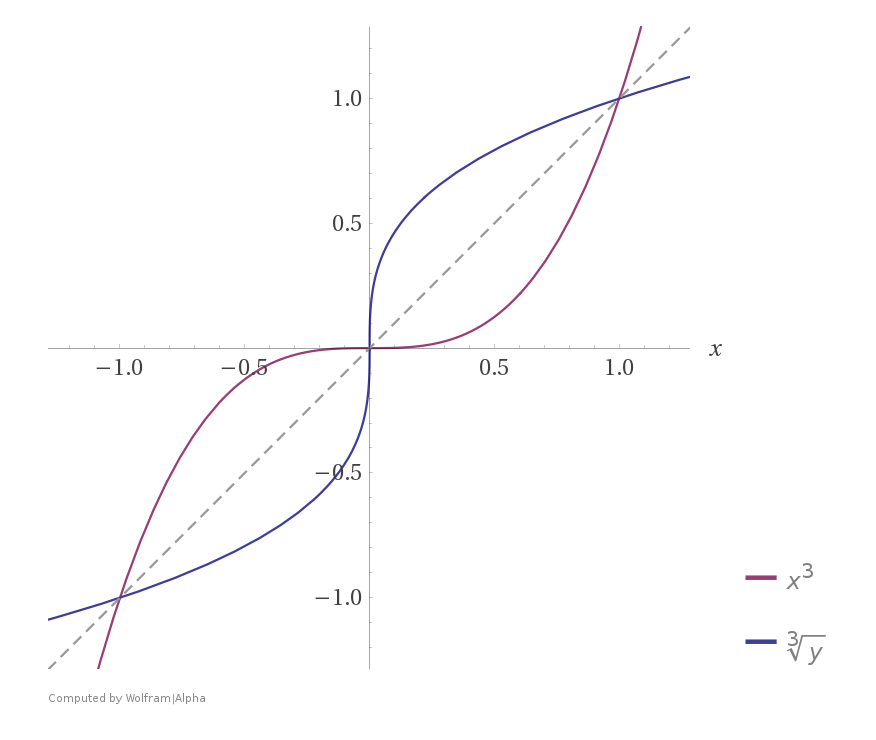
\includegraphics[scale=0.3]{imagens/inversas.png}}
    %\footnotesize{Fonte:~}
  \end{center}
\end{figure}

Como essas duas operações matemáticas são relacionadas e inversas,
existem ainda algumas outras propriedades que ``conectam'' as
potências com as raízes, e ocorrem quando temos potências com
expoentes racionais.


%%%%%%%%%%%%%%%%%%%%%%%%%%%%%%%%%%%%%%%%%%%%%%%%%%%%%%%%%%%%%%%%%%%%%%%%%%%%%%%%%
%%%%%%%%%%%%%%%%%%%%%%%%%%%%%%%%%%%%%%%%%%%%%%%%%%%%%%%%%%%%%%%%%%%%%%%%%%%%%%%%%
\subsection{Propriedades da potenciação com expoente racional}
\label{potenciacao-propriedades-racional}

Potência com expoente racional é uma raiz:
\begin{tcolorbox}[ams equation]
  \label{eqn:pot_rac1}
  a^{\frac{m}{n}} = \left(\sqrt[n]{a}\right)^m = \sqrt[n]{a^m}\quad (n
  \in \mathbb{N}, m \in \mathbb{Z})
\end{tcolorbox}

Algumas vezes é útil entender os expoentes racionais como:
\begin{tcolorbox}[ams equation]
  \label{eqn:pot_rac2}
  a^{\frac{m}{n}} = \left(a^{\frac{1}{n}}\right)^m = a^{\left(\frac{1}{n}\right)(m)}
\end{tcolorbox}

\begin{tcolorbox}[ams equation]
  \label{eqn:pot_rac3}
  a^{\frac{m}{n}} = \left(a^m\right)^{\frac{1}{n}} = a^{(m)\left(\frac{1}{n}\right)}
\end{tcolorbox}




%%%%%%%%%%%%%%%%%%%%%%%%%%%%%%%%%%%%%%%%%%%%%%%%%%%%%%%%%%%%%%%%%%%%%%%%%%%%%%%%%
%%%%%%%%%%%%%%%%%%%%%%%%%%%%%%%%%%%%%%%%%%%%%%%%%%%%%%%%%%%%%%%%%%%%%%%%%%%%%%%%%
%%%%%%%%%%%%%%%%%%%%%%%%%%%%%%%%%%%%%%%%%%%%%%%%%%%%%%%%%%%%%%%%%%%%%%%%%%%%%%%%%
\section{Racionalização de denominadores (ou numeradores)}
\label{racionalizacao}

Em muitos cálculos é conveniente remover as raízes do denominador (e,
em algumas vezes, do numerador). O processo de remover uma raiz de um
denominador é chamado de \emph{racionalização do denominador} (e o
processo de remover uma raiz de um numerador é chamado de
\emph{racionalização do numerador}).

Se uma raiz está isolada no denominador:
\begin{tcolorbox}[ams equation]
  \label{eqn:racionalizacao1}
  \frac{a}{\sqrt{b}} = \frac{a}{\sqrt{b}}\times\frac{\sqrt{b}}{\sqrt{b}} = \frac{a\sqrt{b}}{\sqrt{b^{2}}} = \frac{a\sqrt{b}}{b}
\end{tcolorbox}

Se a raiz no denominador tem um índice e o radicando é uma outra potência:
\begin{tcolorbox}[ams equation]
  \label{eqn:racionalizacao2}
  \frac{a}{\sqrt[n]{b^{m}}} = \frac{a}{\sqrt[n]{b^{m}}} \times
  \frac{\sqrt[n]{b^{n-m}}}{\sqrt[n]{b^{n-m}}} = \frac{a\sqrt[n]{b^{n-m}}}{\sqrt[n]{b^{m}}\sqrt[n]{b^{n-m}}} = \frac{a\sqrt[n]{b^{n-m}}}{\sqrt[n]{b^{m+n-m}}} = \frac{a\sqrt[n]{b^{n-m}}}{\sqrt[n]{b^{n}}} = \frac{a\sqrt[n]{b^{n-m}}}{b}
\end{tcolorbox}

Se a raiz no demonimador faz parte de uma soma (ou subtração), usamos
o conjugado:
\begin{tcolorbox}[ams equation]
  \label{eqn:racionalizacao3}
  \frac{a}{b+\sqrt{c}} = \frac{a}{(b+\sqrt{c})}\times\frac{(b-\sqrt{c})}{(b-\sqrt{c})} = \frac{a(b-\sqrt{c})}{b^{2}-(\sqrt{c})^{2}} = \frac{a(b-\sqrt{c})}{b^{2}-c}
\end{tcolorbox}

A racionalização do numerador é menos freqüênte que a racionalização
do denominador mas, caso seja necessária, pode ser feita utilizando-se
uma das técnicas acima, obviamente aplicadas ao numerador!


%%%%%%%%%%%%%%%%%%%%%%%%%%%%%%%%%%%%%%%%%%%%%%%%%%%%%%%%%%%%%%%%%%%%%%%%%%%%%%%%%
%\subsubsection{Subsubseção}
%\label{subsubetiqueta}


%%%%%%%%%%%%%%%%%%%%%%%%%%%%%%%%%%%%%%%%%%%%%%%%%%%%%%%%%%%%%%%%%%%%%%%%%%%%%%%%%
%%%%%%%%%%%%%%%%%%%%%%%%%%%%%%%%%%%%%%%%%%%%%%%%%%%%%%%%%%%%%%%%%%%%%%%%%%%%%%%%%
%%%%%%%%%%%%%%%%%%%%%%%%%%%%%%%%%%%%%%%%%%%%%%%%%%%%%%%%%%%%%%%%%%%%%%%%%%%%%%%%%
%%%%%%%%%%%%%%%%%%%%%%%%%%%%%%%%%%%%%%%%%%%%%%%%%%%%%%%%%%%%%%%%%%%%%%%%%%%%%%%%%
%%%%%%%%%%%%%%%%%%%%%%%%%%%%%% TERMINA O DOCUMENTO %%%%%%%%%%%%%%%%%%%%%%%%%%%%%%
%%%%%%%%%%%%%%%%%%%%%%%%%%%%%%%%%%%%%%%%%%%%%%%%%%%%%%%%%%%%%%%%%%%%%%%%%%%%%%%%%
%%%%%%%%%%%%%%%%%%%%%%%%%%%%%%%%%%%%%%%%%%%%%%%%%%%%%%%%%%%%%%%%%%%%%%%%%%%%%%%%%
%%%%%%%%%%%%%%%%%%%%%%%%%%%%%%%%%%%%%%%%%%%%%%%%%%%%%%%%%%%%%%%%%%%%%%%%%%%%%%%%%
%%%%%%%%%%%%%%%%%%%%%%%%%%%%%%%%%%%%%%%%%%%%%%%%%%%%%%%%%%%%%%%%%%%%%%%%%%%%%%%%%
\end{document}









